\subsection{Principles of Cryptography}

\begin{itemize}
  \item Confidentiality --- only the sender and intended recipient should be able to understand the message content
  \item End-point authentication --- the sender and receiver wish to confirm the identity of the other
  \item Message integrity --- the sender and receiver wish to ensure the message is not altered without detection
  \item Access and availability --- services must be accessible and available to users
\end{itemize}

The sender and receiver may be users, applications, servers or routers.
Malicious parties may attempt to eavesdrop (intercept messages), actively insert messages into the connection (man-in-the-middle attack), impersonate (fake or spoof the source address or any other field in a packet), hijack an ongoing connection by replacing the sender or receiver, or deny service (prevent it from being used by others by overloading resources, for example).

A plaintext message \(m\) is encrypted with a key \(K_A\) to produce a ciphertext \(\functionsub{K}{A}{m}\).
The ciphertext is decrypted with the key \(K_B\) to reproduce the plaintext message \(m = \functionsub{K}{B}{\functionsub{K}{A}{m}}\).

The two main types of encryption schemes are
\begin{itemize}
  \item symmetric key systems --- sender and receiver keys are identical and secret, and
  \item public key systems --- one key is known to the whole world and the other key is known only to the sender or receiver (but not both).
\end{itemize}

\subsection{Symmetric Key Cryptography}

\begin{figure}[htp]
  \centering
  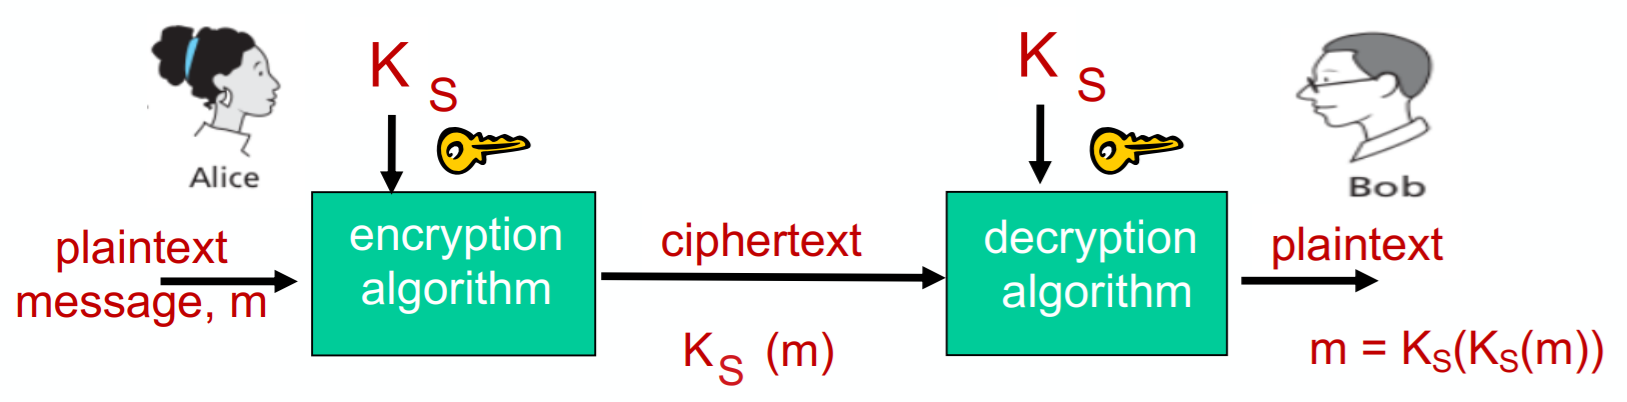
\includegraphics[width=12cm]{unit-20/figures/alice-bob-symmetric.png}
  \caption*{Symmetric key cryptography.}
\end{figure}

With symmetric key cryptography, Alice and Bob share the same symmetric key.
The key may be a mapping for a substitution cipher.
A monoalphabetic cipher is used to substitute each letter for another.

An example of symmetric key cryptography is the Data Encryption Standard (DES), which uses a \SI{56}{\bit} symmetric key and acts on \SI{64}{\bit} plaintext input.
There is no known good analytic attack, but the key can be cracked through brute force typically in under a day.
DES can be made more secure using 3DES (three DES encryptions using three different keys).

The DES encryption operations consists of an initial permutation followed by \num{16} rounds of function application that each use a different \SI{48}{\bit} of the key, and a final permutation.

DES was replaced by the Advanced Encryption Standard (AES), which processes data in \SI{128}{\bit} blocks and uses \SIlist[list-final-separator={ or }]{128;192;256}{\bit} keys.
A brute force decryption taking a maximum of one~second on a DES encryption would take a maximum of \num{149}~trillion years on an AES encryption.

\subsection{Public Key Cryptography}

Symmetric key encryption requires the sender and receiver to know a shared secret key.
This can be difficult to achieve, particularly if the sender and receiver never meet.

Public key encryption does not require the sender and receiver to share a secret key.
The public encryption key is known to all, but the private decryption key is known only to the receiver.

\begin{figure}[htp]
  \centering
  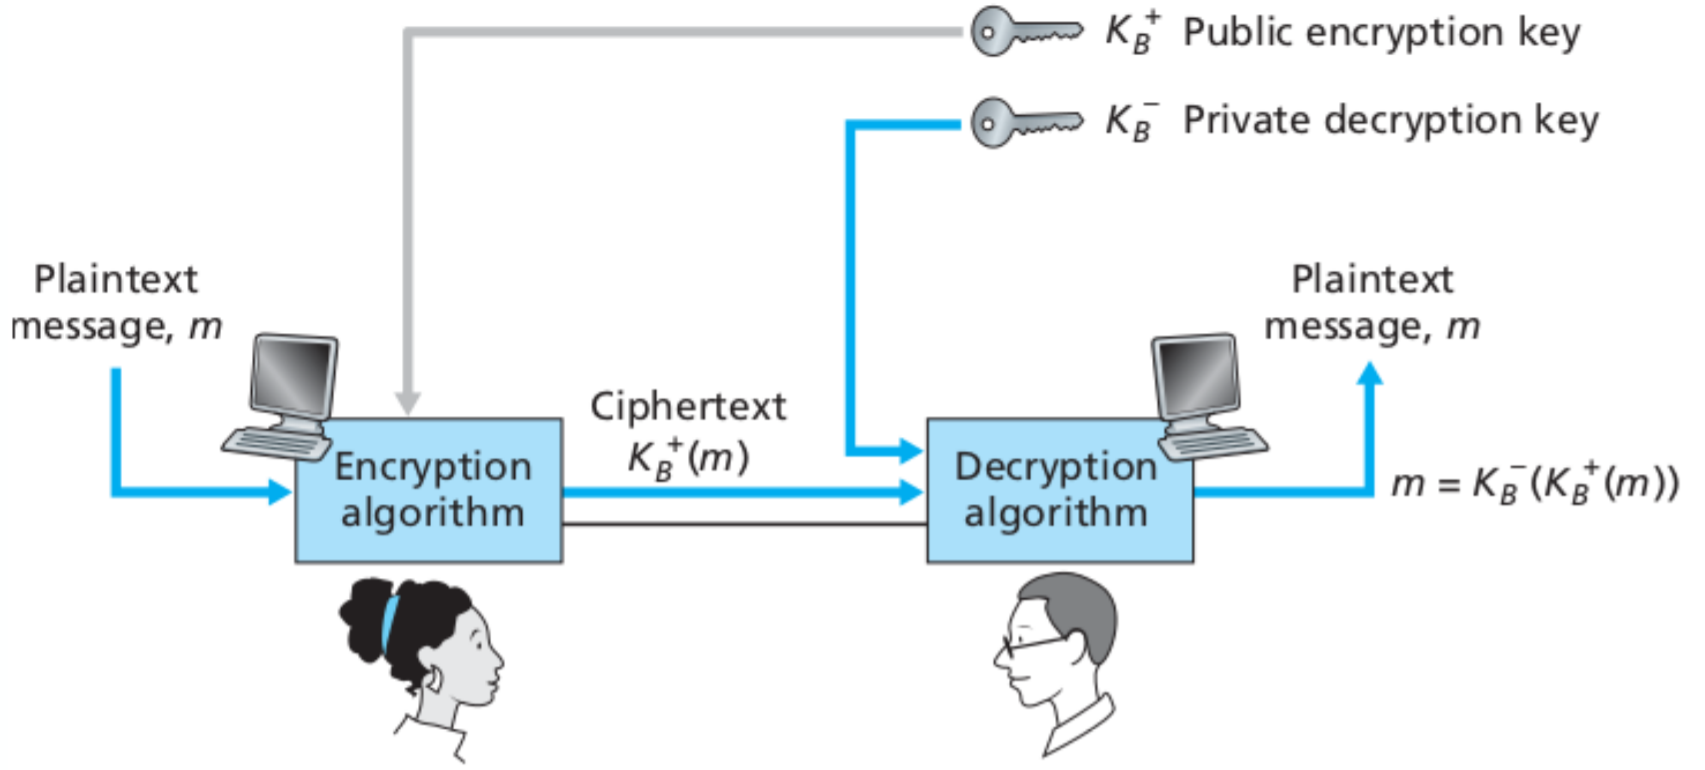
\includegraphics[width=12cm]{unit-20/figures/alice-bob-public.png}
  \caption*{Public key cryptography.}
\end{figure}

Public key encryption requires an encryption key \(K_B^+\) and a decryption key \(K_B^-\) such that \(\functionsubsup{K}{B}{-}{\functionsubsup{K}{B}{+}{m}} = m\).
Given a public key \(K_B^+\), it should be impossible to compute the private key \(K_B^-\).

\subsubsection{Rivest, Shamir, Adelson (RSA) Encryption}

An example of public key encryption is the Rivest, Shamir, Adelson (RSA) algorithm, which uses modular arithmetic.

\begin{align*}
  \left(\left(a \textup{mod} n\right) + \left(b \textup{mod} n\right)\right) \textup{mod} n = \left(a + b\right) \textup{mod} n \\
  \left(\left(a \textup{mod} n\right) - \left(b \textup{mod} n\right)\right) \textup{mod} n = \left(a - b\right) \textup{mod} n \\
  \left(\left(a \textup{mod} n\right) \times \left(b \textup{mod} n\right)\right) \textup{mod} n = \left(a \times b\right) \textup{mod} n \\
\end{align*}

Thus, a similar identity can be constructed for \(\left(a \textup{mod} n\right)^d\).

\begin{equation*}
  \left(a \textup{mod} n\right)^d \textup{mod} n = a^d \textup{mod} n \\
\end{equation*}

A message is simply a bit pattern that can be uniquely represented by an integer.
Thus, the message \(m\) can be encrypted by encrypting its corresponding integer.
The resulting integer is the ciphertext.

\begin{figure}[htp]
  \centering
  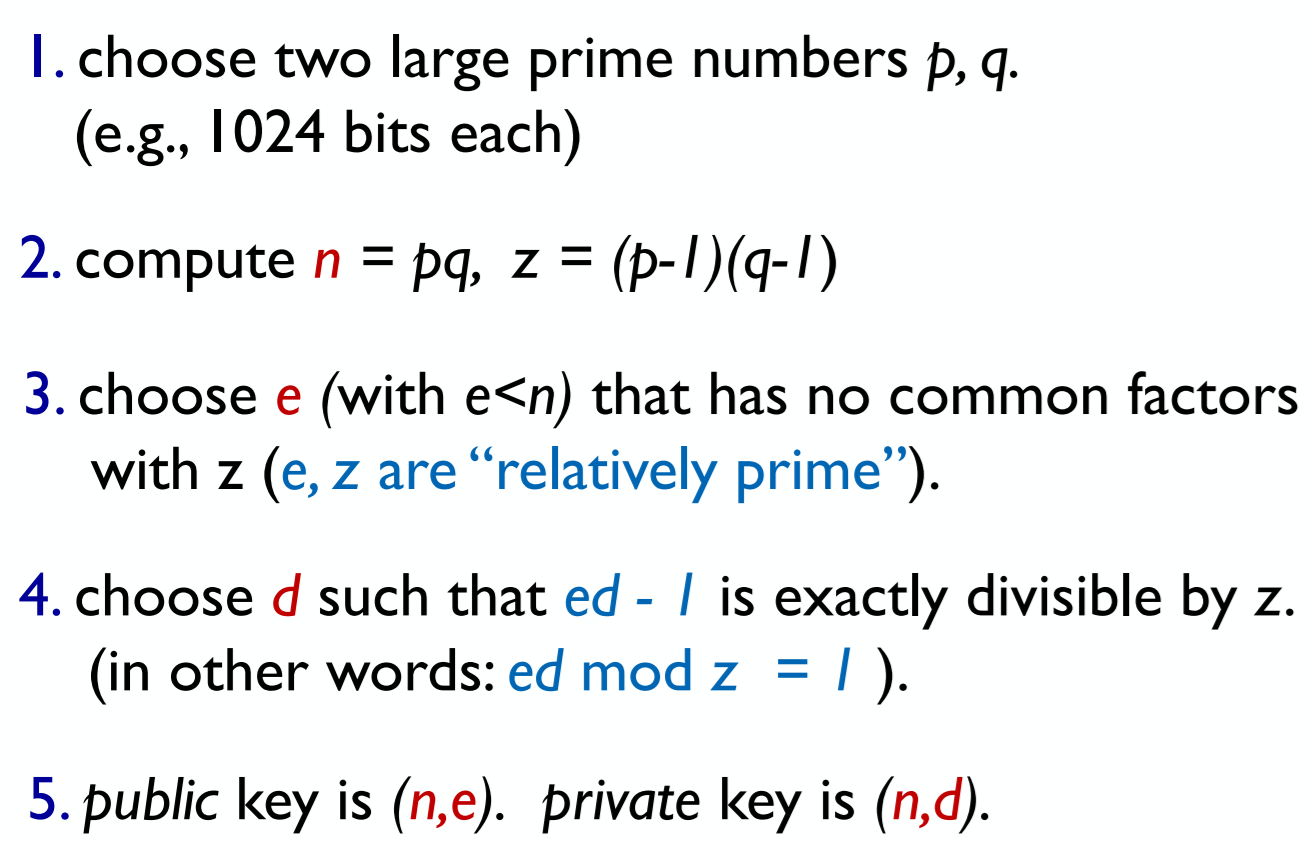
\includegraphics[width=10cm]{unit-20/figures/rsa.png}
  \caption*{The RSA public and private key pair creation algorithm.}
\end{figure}

To encrypt the message \(m\) to ciphertext \(c\), compute \(c = m^e \textup{mod} n\).
To decrypt the ciphertext \(c\), compute \(m = c^d \textup{mod} n\).

\begin{equation*}
  m = \left(m^e \textup{mod} n\right)^d \textup{mod} n
\end{equation*}

\begin{figure}[htp]
  \centering
  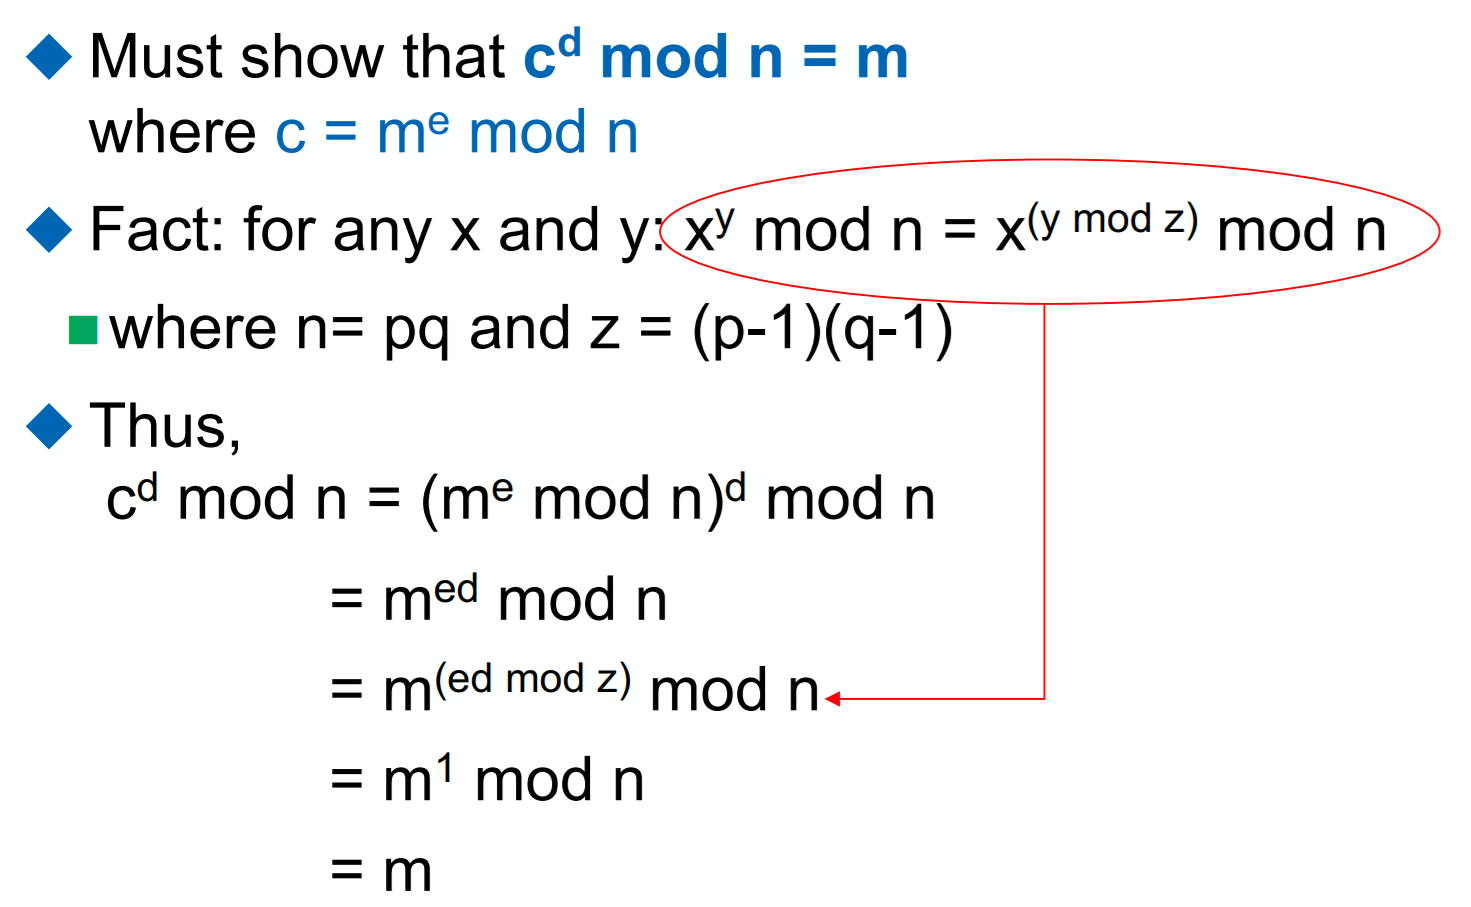
\includegraphics[width=10cm]{unit-20/figures/rsa-proof.png}
  \caption*{Proof of the RSA algorithm.}
\end{figure}

\begin{figure}[htp]
  \centering
  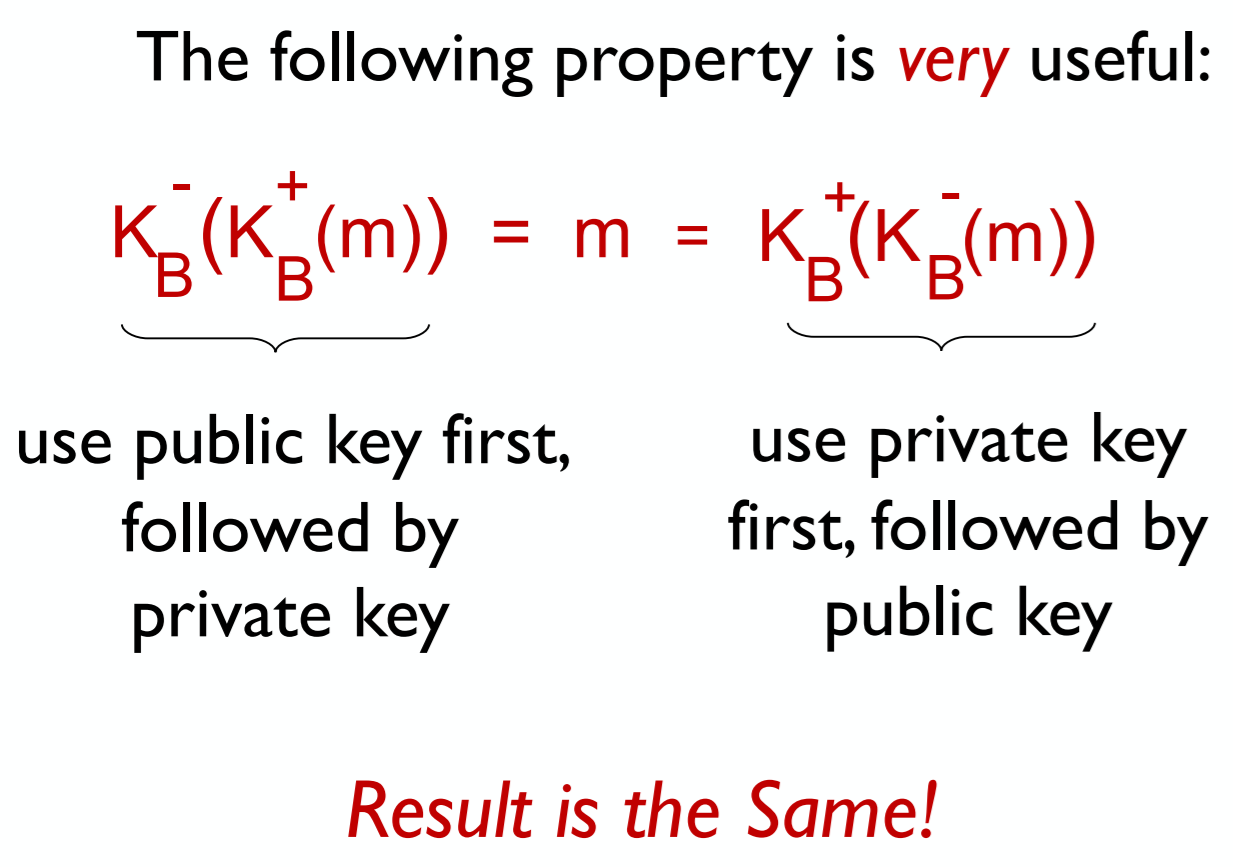
\includegraphics[width=8cm]{unit-20/figures/rsa-associativity.png}
  \caption*{Associativity of RSA encryption.}
\end{figure}

\begin{figure}[htp]
  \centering
  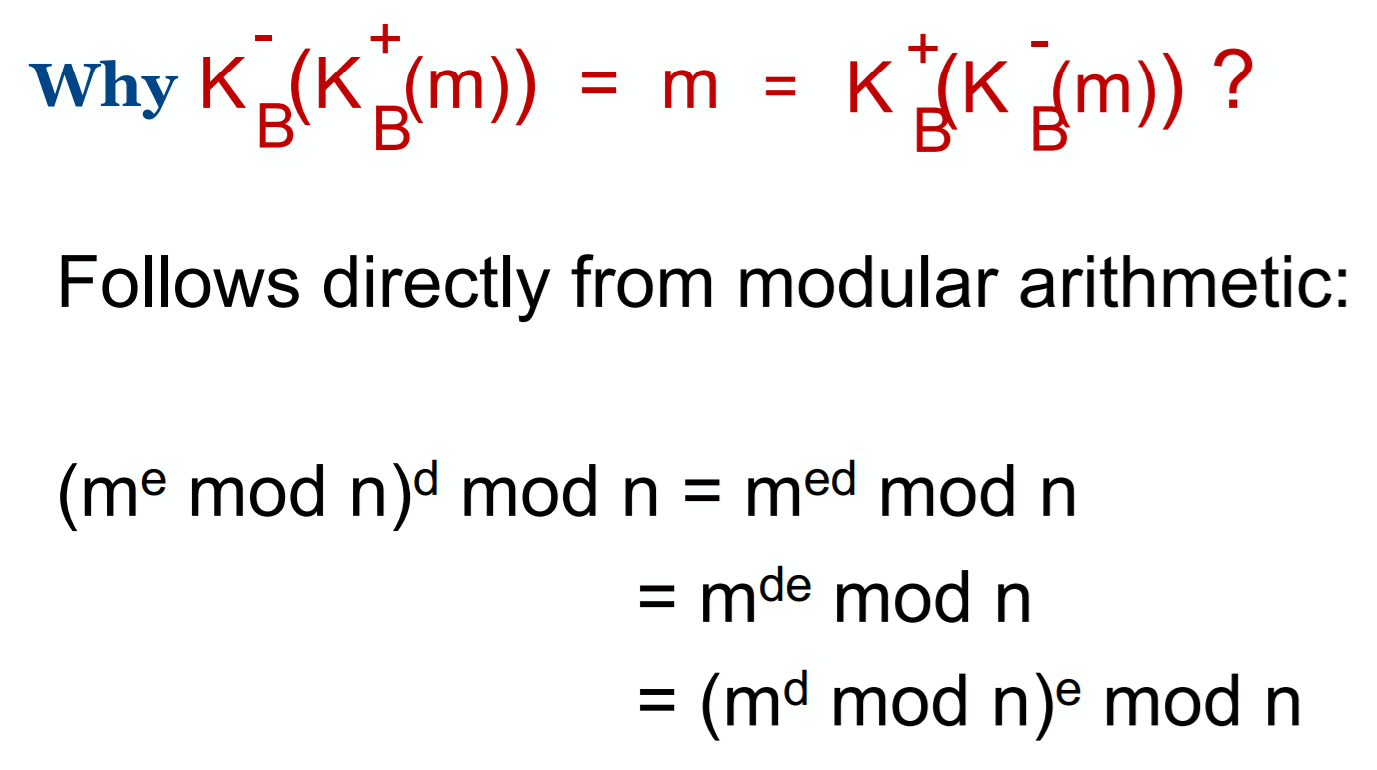
\includegraphics[width=8cm]{unit-20/figures/rsa-associativity-proof.png}
  \caption*{Proof of the associativity of RSA encryption.}
\end{figure}

RSA is secure since it is impossible to determine \(d\) of the private key from \(n\) and \(e\) of the public key.
This would require finding factors of \(n\) without knowing the two factors \(p\) and \(q\).
Factoring a large number is very difficult.

\subsubsection{RSA Session Keys}

The exponentiation required by RSA is computationally intensive.
Thus, RSA is significantly slower than DES\@.
Public key cryptography, such as RSA, is used to establish a secure connection, through which a symmetric session key is established for encrypting data.
Once the sender and receiver have the symmetric key, it is used for communication.
